%\author[1,*]{Jan Szymenderski}
%\author[2,**]{Przemysław Sałapata}
%
%\affil[1]{Politechnika Poznańska, Wydział Elektryczny, pl. Marii Skłodowskiej-Curie 5, 60-965 Poznań}
%\affil[*]{e-mail: jan.szymenderski@put.poznan.pl}
%\affil[**]{e-mail: przemyslaw.salapata@student.put.poznan.pl}



\documentclass{MSRarticle}
\usepackage[T1]{fontenc}
\usepackage[utf8]{inputenc}%zmieniłem na utf8
\usepackage{array}
\usepackage{amstext}
\usepackage{graphicx}
\usepackage{esint}
\usepackage{lettrine}
\usepackage{hyperref}
\usepackage{url}
\usepackage{balance}

\usepackage{verbatim}
\usepackage{smartdiagram}

\usepackage{tikz}
\usepackage{pgfplots}
%\usepackage{showframe}
%\usepackage{fancyhdr}
%\usepackage[bottom]{footmisc}

\DeclareCaptionLabelSeparator{hskip}{.\hskip 4px}
\usepackage[figurename=Rys.\hskip -1.75px,labelsep=hskip ]{caption}

% Input the Heading information:
\Journal{MEASUREMENT SCIENCE REVIEW, \textbf{19}, (2019), No.~x, p1--p2}
\Doi{10.1515/msr-2019-00xx}

% !!! For PDF LaTeX use this version of the MSR HEAD:
%\MSR_Head{MSRhead.pdf}

% Otherwise (for laTeX using PostScript) use the default setup or use this:
%\MSR_Head{MSRhead.eps} 


\setcounter{page}{101}

\begin{document}

\title{Projektowanie geometrii sensorów piezoelektrycznych - elektryczna odpowiedź elementu piezoelektrycznego na wymuszenie mechaniczne }

%\Subtitle{Short Communication}

\author{Jan Szymenderski$^{1,2}$, Przemysław Sałapata$^{1,3}$, Łukasz Gierz$^{1,4}$}

%\affil[1]{Politechnika Poznańska, Wydział Elektryczny, pl. Marii Skłodowskiej-Curie 5, 60-965 Poznań}
%\affil[*]{e-mail: jan.szymenderski@put.poznan.pl}
%\affil[**]{e-mail: przemyslaw.salapata@student.put.poznan.pl}


\Address{$^{1}$Politechnika Poznańska, Wydział Elektryczny, pl. Marii Skłodowskiej-Curie 5, 60-965 Poznań,\\ \protect\href{mailto:jan.szymenderski@put.poznan.pl}{$^{2}$jan.szymenderski@put.poznan.pl}
\\ \protect\href{mailto:przemyslaw.salaptata@student.put.poznan.pl}{$^{3}$przemyslaw.salaptata@student.put.poznan.pl}\\ \protect\href{mailto:lukasz.gierz@put.poznan.pl}{$^{4}$lukasz.gierz@put.poznan.pl}\\}

%TODO
\Abstract{Do napisania streszczenie artykułu.}
%TODO
%\begin{abstract}
%Do napisania streszczenie artykułu.
%%Tutaj streszczenie
%\end{abstract}

\Keywords{Magnetic measurement, imaging, magnetic susceptibility, calculation, microwave frequencies.}

\maketitle

\section{Wprowadzenie}
\label{sec:introduction}

TODO
Do napisania wprowadzenie. Zjawisko piezoelektryczne. Artykuł ma pokazać metodykę projektowania sensorów na konkretnym przykładzie.

\href{http://www.google.com}{przykład linka Google}
\section{Założenia prowadzonych badań}
\label{sec:assumptions}

%\subsection{Wymagania konstrukcyjne}
Źródłem wymuszeń mechanicznych są owalne ciała (bryły sztywne) o masie $m_s=0.03\div1.10 g$ poruszające się torem ruchu przedstawionym na Rys.\ref{fig:route}. Tor wykonany jest ze stalowej rury i w obszarze A (patrz: Rys.\ref{fig:route}) następuje sprężysty kontakt ze ścianą toru. Należy nadmienić, że w obszar A uderza 98\% poruszających się ciał. W odrębnych badaniach ustalono również, że prędkość ciała w momencie kontaktu wynosi $v_s=3.0\div7.0$ $\frac{m}{s}$. Wymuszenia mogą pojawiać się minmalnie w odstępach $T_{smin}=TODO$.

\begin{figure}[htbp]
\centering
\fbox{TUTAJ RYSUNEK TORU RUCHU ZIARNA}%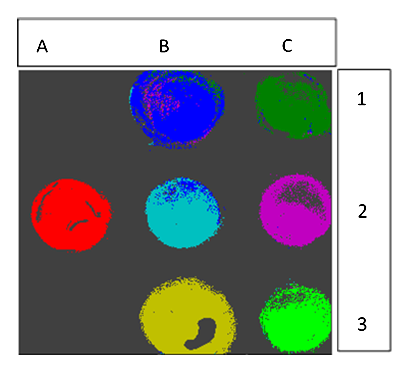
\includegraphics[width=\linewidth]{sample}}
\caption{Zakładany tor lotu ciała fizycznego}
\label{fig:route}
\end{figure}

Założono, że miejscem montażu przetwornika jest obszar A na Rys.\ref{fig:route}, który stanowi okrąg o średnicy $d_p=TODO mm$. Dodatkowo promień ugięcia płaszczyzny A wynosi $R_A=TODOmm$, a kąt padania ciała na tę powierzchnię $\delta_p=135^{\circ}$. 

Tak ściśle i ciekawie przedstawione założenia stały się dobrym punktem wyjścia do szerzej rozumianych badań. Artykuł na naszkicowanym już przykładzie ukazuje zależność odpowiedzi elektrycznej wybranych przetworników PVDF z energią wymuszenia mechanicznego a przede wszystkim kostrukcją (zwaną także geometrią) układu.
\section{Metodyka badań}
\label{sec:exp_methods}
Jednym z najważniejszych aspektów badań było ich zaprojektowanie. Tu najlepiej sprawdza się metoda burzy mózgów. Można rzec, że była ona nieodłącznym elementem każdego etapu badań. Na Rys.\ref{fig:workflow}. przedstawiono efekt prac nad sposobem realizacji celu eksperymentów. Ważniejszym etapom poświęcono osobny akapit artykułu. Natomiast niewymagającym komentarza przypisano krótkie wyjaśnienie.

\begin{figure}[htbp]
\centering
\smartdiagramset{back arrow disabled=true}
\smartdiagram[descriptive diagram]{
{Założenia, Ustalenie założeń konstrukcyjnych czujnika},
{Analiza, Separacja założeń mających wpływ na badany układ. },
{Stanowisko, Budowa układu pozwalającego na odizolowanie czynników zewnętrznych oraz zapewniającego odpowiednią regulację energii zderzenia.(patrz: \ref{sec:test_stand})},
{Czujniki, Wybór zestawu i rodzaju przetworników do badań.},
{Selekcja czujnika, Badania prowadzące do wyboru optymalnego czujnika.(patrz: \ref{sec:sensor_selection})},
{Optymalizacja układu, Eksperymenty prowadzące do optymalizacji przestrzennego wyglądu czujnika. Kontrola czujników odrzuconych w kroku poprzednim i ewentualny powrót do kroku poprzedniego. (patrz: \ref{sec:construction_optymization})},
{Analiza, Analiza pozyskanych danych.(patrz: \ref{sec:conclusion})},
}
\caption{Infografika obrazująca metodykę prowadzonych badań.}
\label{fig:workflow}
\end{figure}

\section{Stanowisko badawcze}
\label{sec:test_stand}

Konstrukcję stanowiska badawczego uzależniono od kilku czynników:
%lista punktowana
\begin{itemize}
\item prostota budowy
\item możliwość wymiany modelu przetwornika (patrz: Rys.\ref{fig:test_stand})
\item łatwa zmiana mocowania przetwornika
\item możliwość regulacji energii wymuszenia mechanicznego
\end{itemize}

\begin{figure}[htbp]
\centering
\fbox{TUTAJ PROJEKT STANOWISKA}%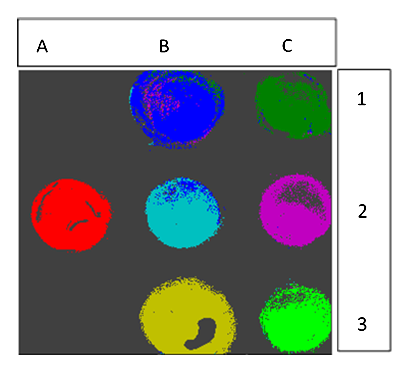
\includegraphics[width=\linewidth]{sample}}
\caption{Projekt stanowiska badawczego.}
\label{fig:test_stand}
\end{figure}

\begin{figure}[htbp]
\centering
\fbox{TUTAJ ZDJĘCIE STANOWISKA}%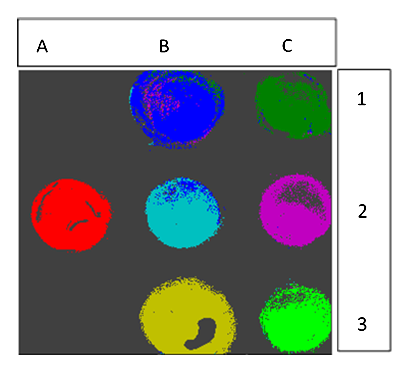
\includegraphics[width=\linewidth]{sample}}
\caption{Realizacja stanowiska badawczego.}
\label{fig:test_stand_photo}
\end{figure}
%sekcja wyboru czujnika piezo
\section{Selekcja czujnika}
\label{sec:sensor_selection}
Równolegle z pracami nad stanowiskiem badawczym przeprowadzono przegląd dostępnych na rynku przetworników piezoelektrycznych. Uwagę skoncentrowano przede wszystkim na przetwornikach PVDF\cite{PVDF:15}\footnote{Polifluorek winylidenu - materiał piezoelektryczny charakteryzujący się elastycznością.} Do badań wybrano 6 konkretnych produktów (patrz: Rys.\ref{fig:sensors}.):

\begin{enumerate}
\item Czujnik TODO
\item Czujnik TODO
\item Czujnik TODO
\item Czujnik TODO
\item Czujnik TODO
\item Czujnik TODO
\end{enumerate}


\begin{figure}[htbp]
\centering
\fbox{TUTAJ ZDJĘCIE CZUJNIKÓW}%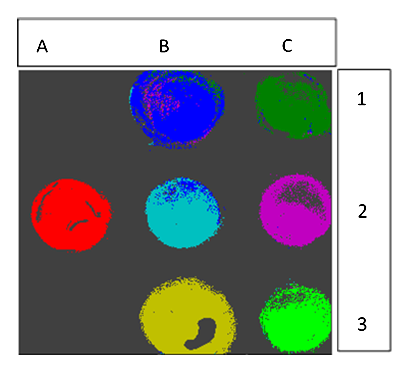
\includegraphics[width=\linewidth]{sample}}
\caption{Badane przetworniki piezoelektryczne.}
\label{fig:sensors}
\end{figure}

Aby dokonać selekcji przetwornika wybrano najprostszy układ geometryczny (patrz: Rys. \ref{fig:sensor_sel_geometry})

\begin{figure}[htbp]
\centering
\fbox{TUTAJ RYSUNEK GEOMETRII CZUJNIKA }%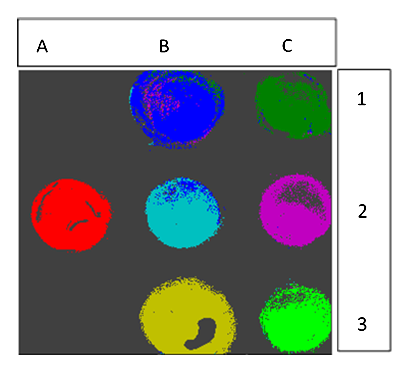
\includegraphics[width=\linewidth]{sample}}
\caption{Konstrukcja pozwalająca na selekcję przetwornika piezoelektrycznego.}
\label{fig:sensor_sel_geometry}
\end{figure}


\section{Optymalizacja układu geometrycznego}
\label{sec:construction_optymization}
\begin{figure}[htbp]
\centering
\fbox{BADANE UKŁADY GEOMETRYCZNE - szkic }%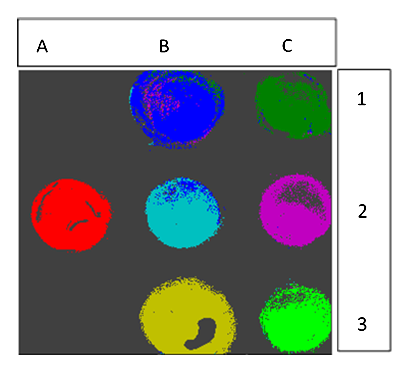
\includegraphics[width=\linewidth]{sample}}
\caption{Szkic badanych układów konstrukcyjnych sensorów piezoelektrycznych.}
\label{fig:construct_scetch}
\end{figure}
Niełatwe rozważania na temat kierunku badań dotyczących konstrukcji sensora zaowocowały ustaleniami o konieczności zbadania przetwornika:
\begin{enumerate}
\item belkowego ze względu na możliwość odniesienia się do istniejącej literatury(patrz: A na Rys.\ref{fig:construct_scetch}),
\item o kształcie rury z powodu przeznaczenia konstruowanego przetwornika (patrz: B na Rys.\ref{fig:construct_scetch}),
\end{enumerate}

%\section{Wyznaczenie charakterystyk}
\section{Podsumowanie}
\label{sec:conclusion}

%przykłady z szablonu
%\subsection{Sample Table}

Table \ref{tab:shape-functions} shows an example table.

\begin{table}[htbp]
\centering
\caption{\bf Shape Functions for Quadratic Line Elements}
\begin{tabular}{ccc}
\hline
local node & $\{N\}_m$ & $\{\Phi_i\}_m$ $(i=x,y,z)$ \\
\hline
$m = 1$ & $L_1(2L_1-1)$ & $\Phi_{i1}$ \\
$m = 2$ & $L_2(2L_2-1)$ & $\Phi_{i2}$ \\
$m = 3$ & $L_3=4L_1L_2$ & $\Phi_{i3}$ \\
\hline
\end{tabular}
  \label{tab:shape-functions}
\end{table}

\section{Sample Equation}

Let $X_1, X_2, \ldots, X_n$ be a sequence of independent and identically distributed random variables with $\text{E}[X_i] = \mu$ and $\text{Var}[X_i] = \sigma^2 < \infty$, and let
\begin{equation}
S_n = \frac{X_1 + X_2 + \cdots + X_n}{n}
      = \frac{1}{n}\sum_{i}^{n} X_i
\label{eq:refname1}
\end{equation}
denote their mean. Then as $n$ approaches infinity, the random variables $\sqrt{n}(S_n - \mu)$ converge in distribution to a normal $\mathcal{N}(0, \sigma^2)$.

\section{Sample Algorithm}

Algorithms can be included using the commands as shown in Algorithm \ref{alg:euclid}.

\begin{algorithm}
\caption{Euclid’s algorithm}\label{alg:euclid}
\begin{algorithmic}[1]
\Procedure{Euclid}{$a,b$}\Comment{The g.c.d. of a and b}
\State $r\gets a\bmod b$
\While{$r\not=0$}\Comment{We have the answer if r is 0}
\State $a\gets b$
\State $b\gets r$
\State $r\gets a\bmod b$
\EndWhile\label{euclidendwhile}
\State \textbf{return} $b$\Comment{The gcd is b}
\EndProcedure
\end{algorithmic}
\end{algorithm}

\section*{Funding Information}
National Science Foundation (NSF) (1263236, 0968895, 1102301); The 863 Program (2013AA014402).

\section*{Acknowledgments}

Formal funding declarations should not be included in the acknowledgments but in a Funding Information section as shown above. The acknowledgments may contain information that is not related to funding:

The authors thank H. Haase, C. Wiede, and J. Gabler for technical support.

\section*{Supplemental Documents}
\emph{Optica} authors may include supplemental documents with the primary manuscript. For details, see \href{http://www.opticsinfobase.org/submit/style/supplementary-materials-optica.cfm}{Supplementary Materials in Optica}. To reference the supplementary document, the statement ``See Supplement 1 for supporting content.'' should appear at the bottom of the manuscript (above the references).

%\bigskip \noindent See \href{link}{Supplement 1} for supporting content.

\section*{References}

For references, you may add citations manually or use BibTeX. E.g. \cite{Zhang:14}.

Note that letter submissions to \emph{Optica} use an abbreviated reference style. Citations to journal articles should omit the article title and final page number; this abbreviated reference style is produced automatically when the \texttt{$\setminus$setboolean\{shortarticle\}\{true\}} option is selected in the template, if you are using a .bib file for your references.

However, full references (to aid the editor and reviewers) must be included as well on an informational page that will not count against page length; again this will be produced automatically if you are using a .bib file and have the \texttt{$\setminus$setboolean\{shortarticle\}\{true\}} option selected.
%przykłady z szablonu

% Bibliography
\bibliography{sample}
%\bibliography{achs_iechad_56_53}

% Full bibliography will be added automatically on a new page for Optics Letters submissions. This command is ignored for journal article submissions.
% Note that this extra page will not count against page length.
%\bibliographyfullrefs{sample}


%Manual citation list
%\begin{thebibliography}{1}
%\bibitem{Zhang:14}
%Y.~Zhang, S.~Qiao, L.~Sun, Q.~W. Shi, W.~Huang, %L.~Li, and Z.~Yang,
 % \enquote{Photoinduced active terahertz metamaterials with nanostructured
  %vanadium dioxide film deposited by sol-gel method,} Opt. Express \textbf{22},
  %11070--11078 (2014).
%\end{thebibliography}

\end{document} 